% BioSystemsSensing.tex

\tikzstyle{LabelObject}=[fill=white,rectangle,align=center]
\tikzstyle{Block}=[rectangle,draw=blue,rounded corners,line width=0.5mm,
  align=center,minimum height=12em,minimum width=32em]

\resizebox{!}{0.4\textwidth}{
	\begin{tikzpicture}[x=1.25cm, y=1.25cm, >=stealth]
		%\draw[help lines,xstep=.5,ystep=.5] (-9,-10) grid (15,3);
		%\foreach \x in {-9,-8,...,15} { \node [anchor=north] at (\x/1,0) {0.\x}; }
		%\foreach \y in {-10,-9,...,3} { \node [anchor=east] at (0,\y/1) {0.\y}; }
	  %
		\begin{scope}
			\node[anchor=center,inner sep=0] (image11) at (0,0)%
				{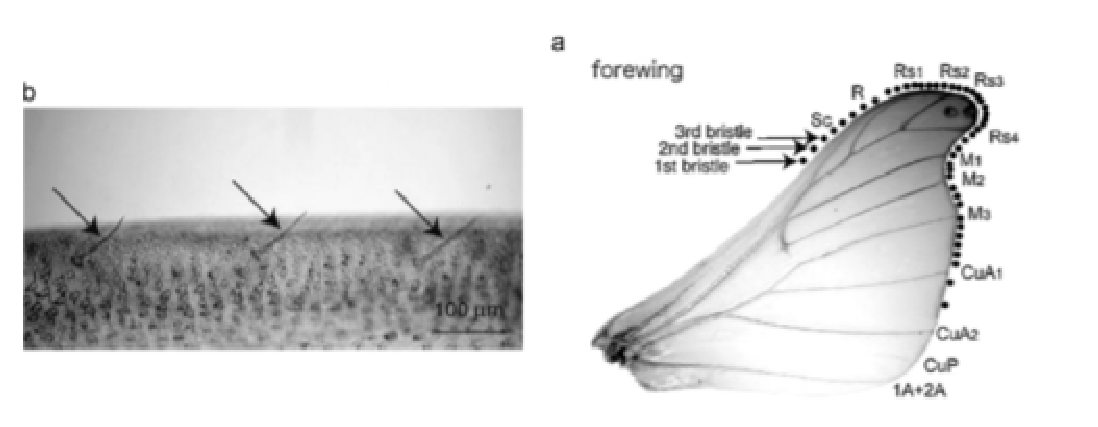
\includegraphics[height=0.25\textwidth]{Yoshida_InsectHairs.eps}};
		\end{scope}
		\begin{scope}
			\node[anchor=center,inner sep=0] (image21) at (0,-4)%
				{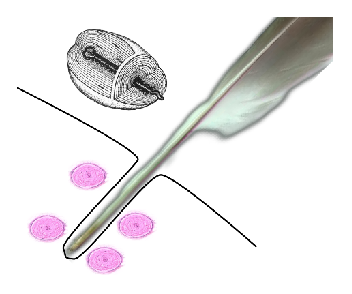
\includegraphics[height=0.25\textwidth]{HerbstCorpuscles.eps}};
		\end{scope}
		\begin{scope}
			\node[anchor=center,inner sep=0] (image31) at (0,-8)%
				{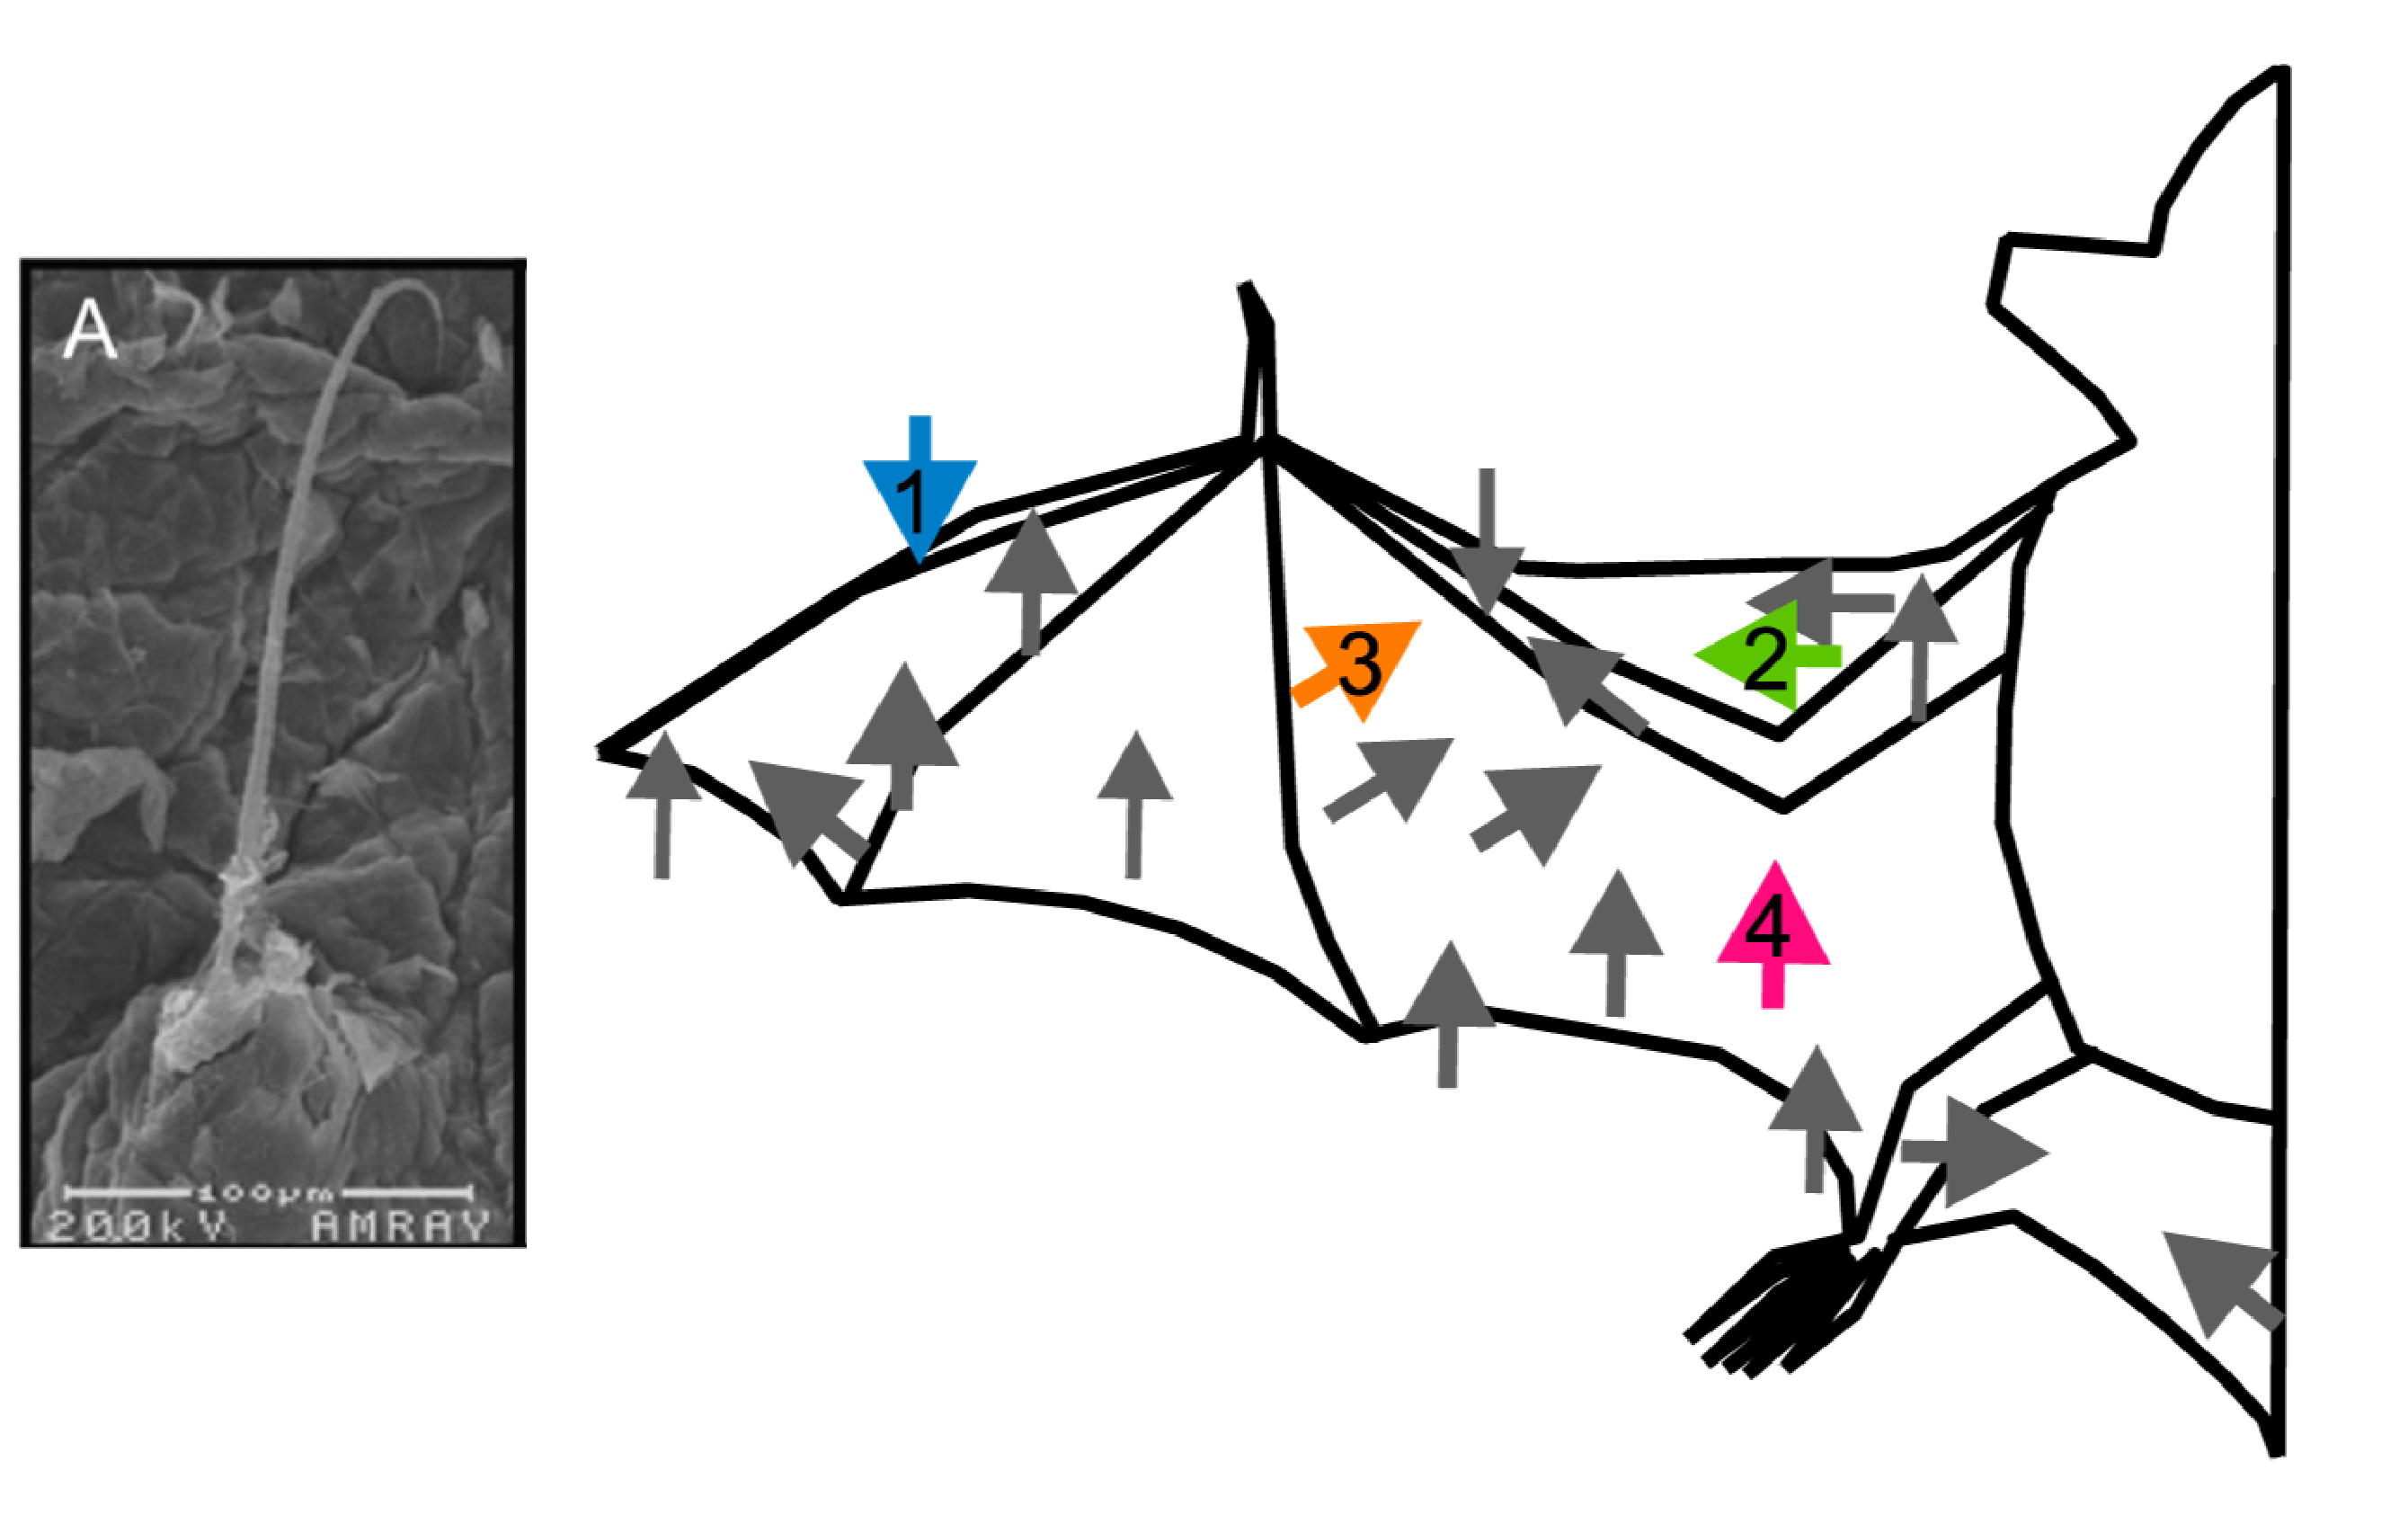
\includegraphics[height=0.25\textwidth]{SterbingDAngelo_BatHairs.eps}};
		\end{scope}
		%
		\begin{scope}
		  \node[anchor=center,inner sep=0] (image12) at (10,0)%
				{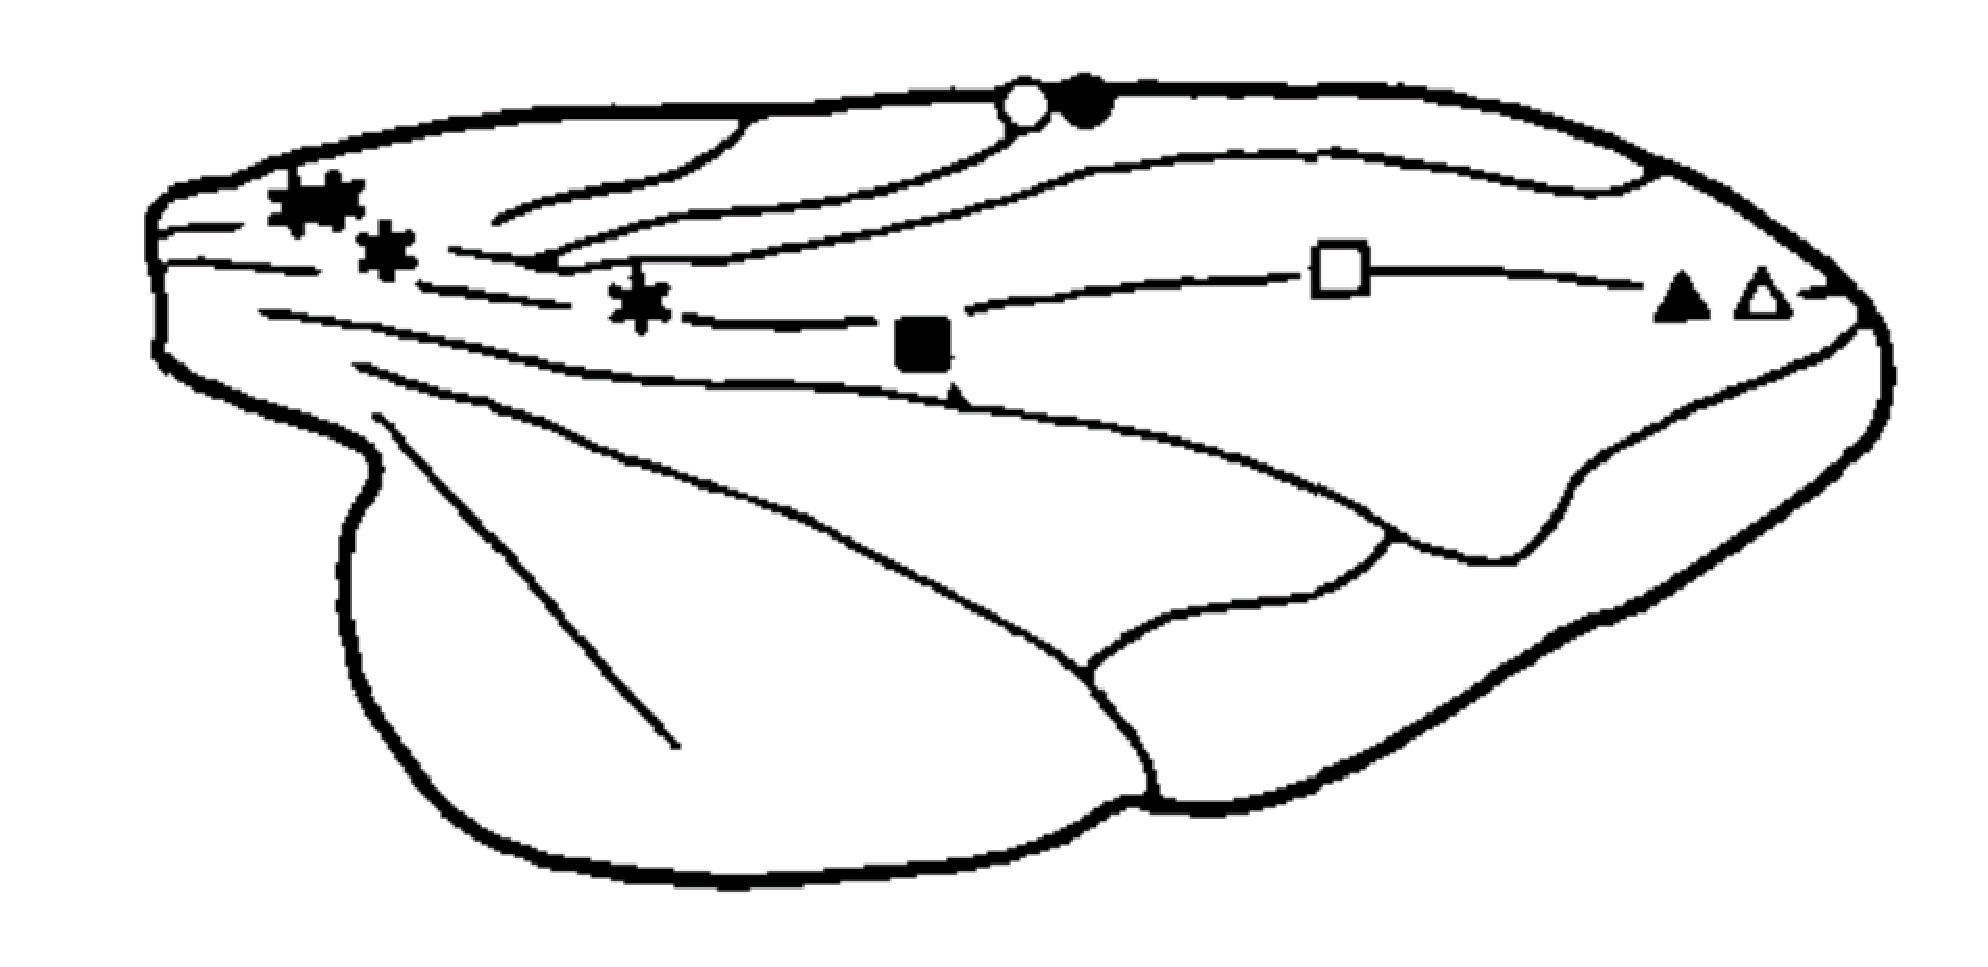
\includegraphics[height=0.25\textwidth]{Dickinson_Fly_CampaniformSensilla.eps}};
		\end{scope}
		\begin{scope}
		  \node[anchor=center,inner sep=0] (image22) at (10,-4)%
				{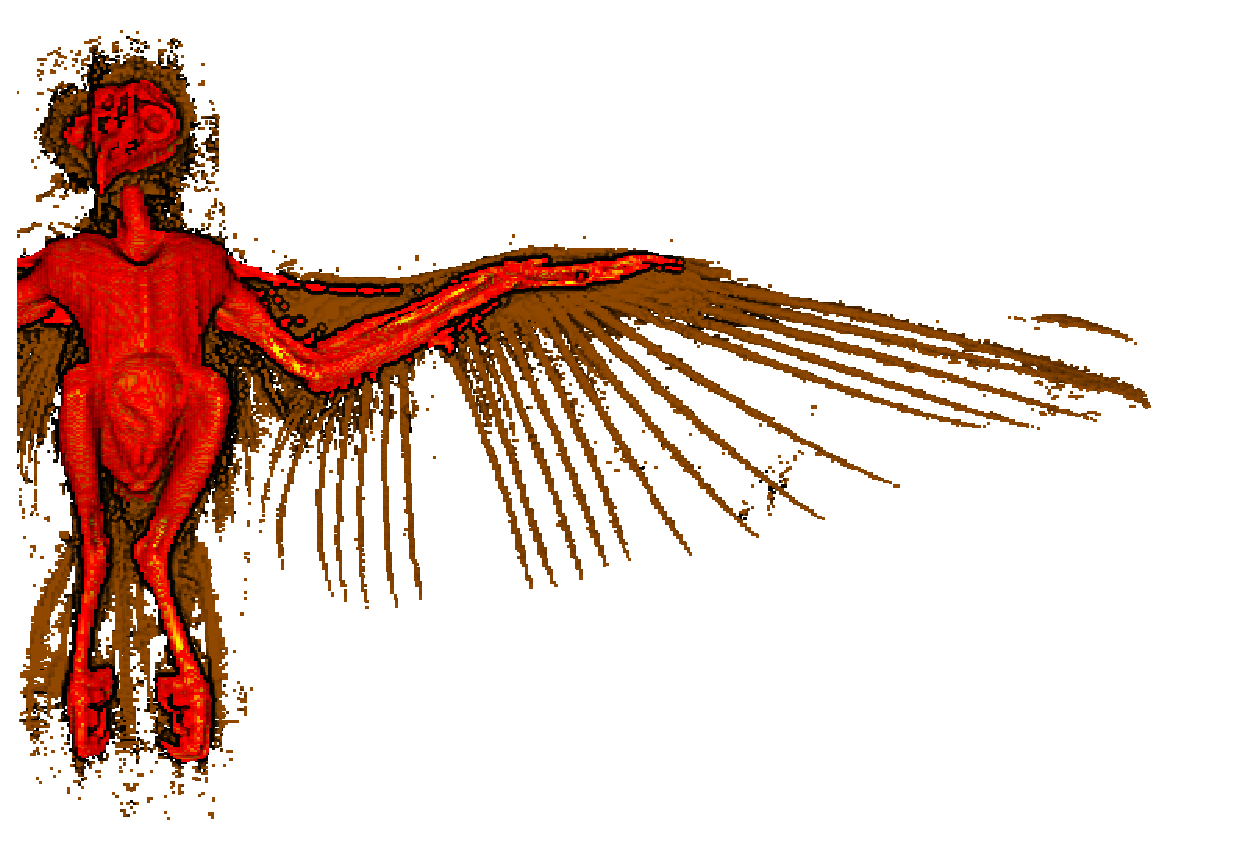
\includegraphics[height=0.25\textwidth]{BarnOwlCT_MuscleFeatherOffset.eps}};
		\end{scope}
		\begin{scope}
		  \node[anchor=center,inner sep=0] (image32) at (10,-8)%
				{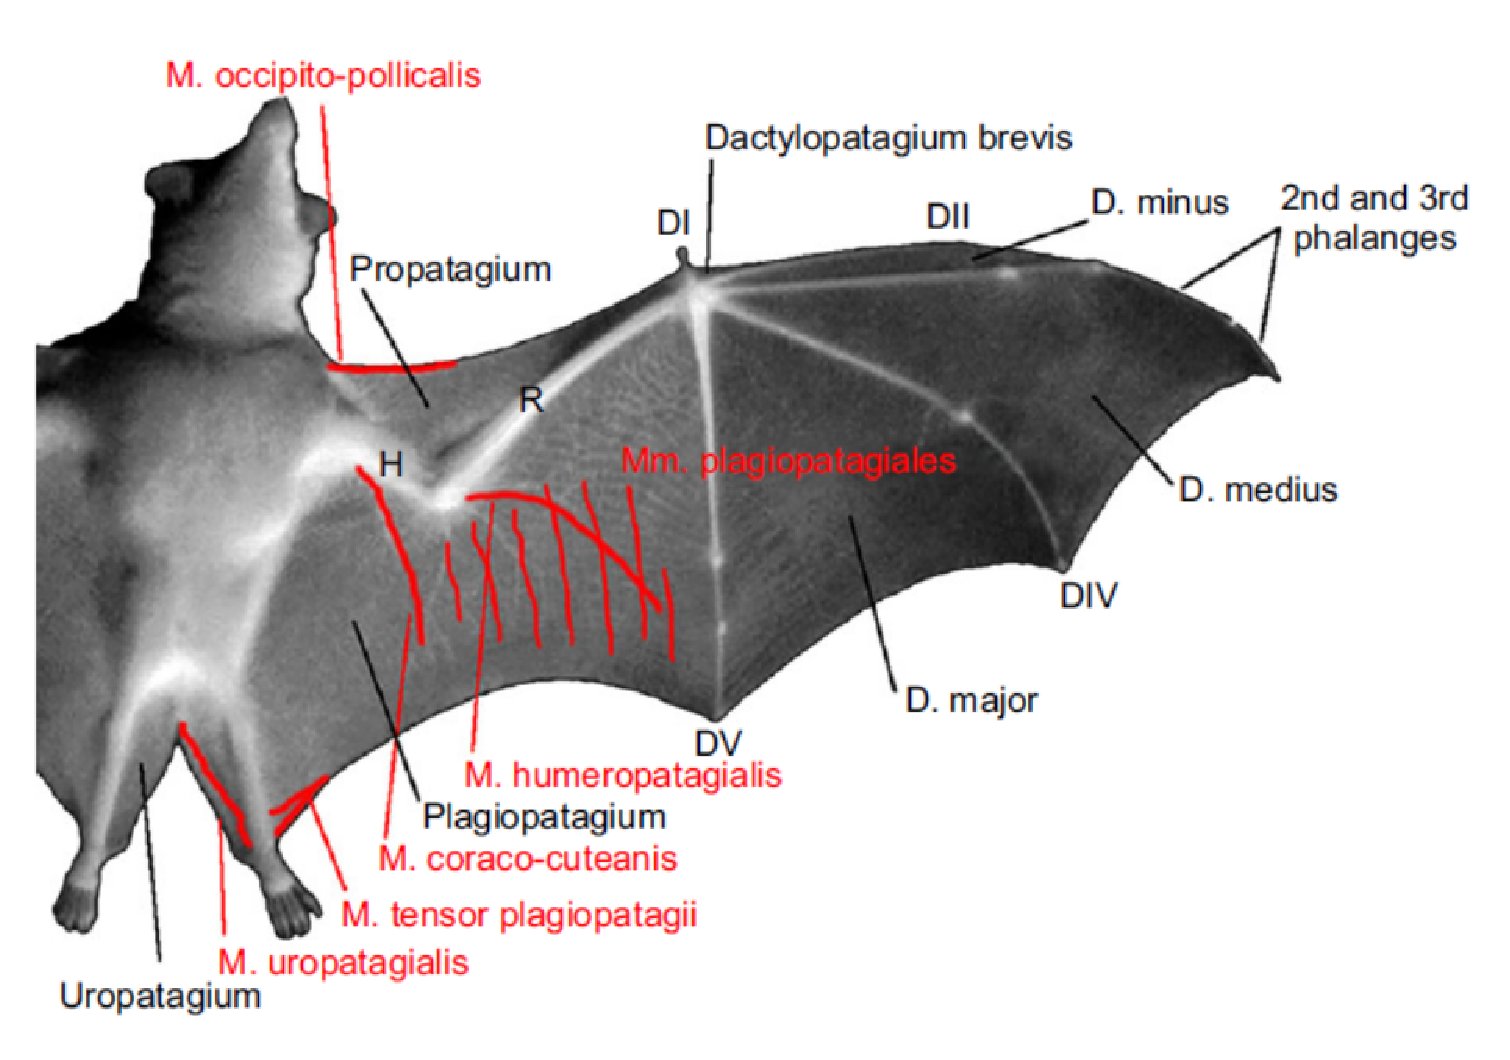
\includegraphics[height=0.25\textwidth]{Bat_MuscleSpindles.eps}};
		\end{scope}
		%
		\draw(image11.north) ++(0,1) node (FlowSens_Label) {\Huge{\bf Flow Sensors}};
		\draw(image12.north) ++(0,1) node (ForceSens_Label) {\Huge{\bf Force Sensors}};
		\draw(image11.west) ++(-6, 0) node (Insects_Label) {\Huge{\bf Insects}};
		\draw(image11.west) ++(-6,-4) node (Birds_Label) {\Huge{\bf Birds}};
		\draw(image11.west) ++(-6,-8) node (Bats_Label) {\Huge{\bf Bats}};
		%
		\draw(image11.north west) ++(2.5,-0.5) node[LabelObject] (InsectHairs_Label) {Silkworm moth: Bristles/Hairs};
		\draw(image11.south west) ++(2.5,0.0) node[gray,LabelObject] (InsectHairsAuthor_Label) {Ai et al. (2010)};
		\draw(image12.east) ++(1,  0) node[LabelObject] (InsectCampSens_Label) {Blowfly:\\Campaniform\\sensilla};
		\draw(image12.east) ++(1, -1) node[gray,LabelObject] (InsectCampSensAuthor_Label) {Dickinson (1990)};
		
		\draw(image21.west) ++(-1,  0) node[LabelObject] (HerbstCorpuscles_Label) {Herbst\\corpuscles};
		\draw(image22.east) ++(1,  0) node[LabelObject] (BirdSpindles_Label) {Muscle\\spindles};
		
		\draw(image31.west) ++(-1,  0) node[LabelObject] (BatHairs_Label) {Hairs};
		\draw(image31.west) ++( 1, -1.5) node[gray,LabelObject] (BatHairsAuthor_Label) {Sterbing-D'Angeloa et al. (2011)};
		\draw(image32.east) ++(1,  0) node[LabelObject] (BatSpindles_Label) {Muscle\\spindles};
		\draw(image32.east) ++(1, -1) node[gray,LabelObject] (BatSpindlesAuthor_Label) {Hedenstrom et al. (2015)};
		
		
		\only<2>{
		  % Sensing system 11
		  \draw(image11) node[Block] (SensSystem11) {};
		}
		\only<3>{
		  % Sensing system 12
		  \draw(image12) +(0.9,0) node[Block] (SensSystem12) {};
		}
		\only<4>{
		  % Sensing system 21
		  \draw(image21) node[Block] (SensSystem21) {};
		}
		\only<5>{
		  % Sensing system 22
		  \draw(image22) +(0.9,0) node[Block] (SensSystem22) {};
		}
		\only<6>{
		  % Sensing system 31
		  \draw(image31) node[Block] (SensSystem31) {};
		}
		\only<7>{
		  % Sensing system 32
		  \draw(image32) +(0.9,0) node[Block] (SensSystem32) {};
		}
		
	\end{tikzpicture}
}